\chapter{Implementazione}
In questa sezione verrà illustrato il porting di Edge Engine da Arduino ESP32 a dispositivi di tipo PC. Al fine di mantenere il prodotto finale slegato dalla piattaforma, si è scelto di utilizzare il compilatore \textbf{g++}, disponibile su dispositivi Windows, Linux e MacOS.\\
In primo luogo verrà discussa l’installazione delle librerie POCO, necessarie per usufruire delle HTTP requests, per poi passare alla modifica del codice preesistente affinché possa essere eseguito sul target desiderato mantenendo però la compatibilità con dispositivi Arduino. In ultimo, verranno mostrati un possibile esempio di utilizzo e la creazione di una libreria vera e propria al fine di permettere una diffusione su più larga scala unita ad una facilità d'uso maggiore.
\section{Librerie POCO}
Come anticipato in precedenza, la prima versione di Edge Engine, in quanto prevista per Arduino, era dotata di due classi wrapper, \textit{Connection} e \textit{APIRest}, adibite alla gestione di risorse hardware e, pertanto, legate alla piattaforma in uso. Di conseguenza, si è resa necessaria la creazione di altre due classi che permettessero di svolgere le stesse funzioni su dispositivi PC. Dal momento che le due classi necessitano di effettuare HTTP requests o di accedere alla rete Internet e l’obbiettivo del progetto è quello di mantenere il più possibile il codice indipentente dalla piattaforma, si è scelto di fare affidamento sulle librerie POCO \cite{POCO}.
\subsection{Installazione}
Le librerie POCO sono un potente strumento C++ multipiattaforma per la creazione di applicazioni basate su rete e Internet che funzionano su desktop, server, dispositivi mobili, IoT e sistemi integrati.\\
L’installazione di queste librerie, tuttavia, si è rivelata più complicata del previsto dal momento che la documentazione riguardante la compilazione delle stesse utilizzando g++ è quasi del tutto assente.\\
\subsubsection{VCPKG, CMake, Conan}
In primo luogo, come da istruzioni del sito POCO, si è tentata l’installazione attraverso il package manager di Windows VCPKG \cite{VCPKG}: un gestore di pacchetti open source multipiattaforma di Microsoft. \\
Nonostante su VCPKG fosse presente il supporto alla compilazione di tali librerie tramite g++, il processo si interrompeva intorno al 70\% a causa del seguente errore:\\
\begin{verbatim}
In file included 
        from C:/mingw/mingw64/x86_64-w64-mingw32/include/mprapi.h:16,
        from C:/mingw/mingw64/x86_64-w64-mingw32/include/iprtrmib.h:12,
        from C:/mingw/mingw64/x86_64-w64-mingw32/include/Iphlpapi.h:15,
        from C:/poco/Foundation/include/Poco/UnWindows.h:33,
        from C:/poco/Foundation/include/Poco/Platform_WIN32.h:22,
        from C:/poco/Foundation/include/Poco/Foundation.h:100,
        from C:/poco/Net/include/Poco/Net/ICMPPacket.h:21,
        from C:\poco\Net\src\ICMPPacket.cpp:15:
C:/poco/Net/include/Poco/Net/ICMPv4PacketImpl.h:72:3: error: expected 
identifier before '(' token
   TIMESTAMP_REQUEST,
   ^~~~~~~~~~~~~~~~~
   
   [...]
   
mingw32-make.exe[2]: *** [Net\CMakeFiles\Net.dir\build.make:679:
Net/CMakeFiles/Net.dir/src/ICMPPacket.cpp.obj] Error 1
mingw32-make.exe[1]: *** [CMakeFiles\Makefile2:530: 
Net/CMakeFiles/Net.dir/all] Error 2
mingw32-make.exe: *** [Makefile:151: all] Error 2

\end{verbatim}
Il secondo tentativo è stato invece effettuato utilizzando CMake \cite{CMake}. CMake è un tool modulare che, con poche e concise istruzioni, è in grado di generare Makefile. CMake dispone di una particolare sintassi comprensiva di moltissime macro ed il loro utilizzo è possibile mediante un apposito file chiamato  \textbf{CMakeLists.txt}. Per la generazione del Makefile e la successiva compilazione del progetto, è necessario eseguire i seguenti comandi:
\begin{verbatim}
mkdir build
cd build
cmake ..
make
\end{verbatim}
Anche in questo caso però, la compilazione si interrompeva attorno al 70\% restituendo lo stesso errore di VCPKG.\\
A seguito dei primi due tentativi falliti, si è scelto di provare a installare le librerie POCO tramite Conan: un package manager open source per lo sviluppo C e C++ che consente ai team di sviluppo di gestire in modo semplice ed efficiente i loro pacchetti e dipendenze tra piattaforme e sistemi di compilazione \cite{Conan}. Il funzionamento di Conan è analogo a quello di VCPKG, ma i file necessari all’installazione delle librerie sono differenti, pertanto ci si sarebbe potuto aspettare un esito differente da quelli passati. Tuttavia, dopo aver seguito le istruzioni specificate dalla guida all'utilizzo, il risultato ottenuto è stato analogo ai precedenti.
\subsubsection{MSYS2}
In ultimo, nonostante non ci fosse alcuna documentazione a riguardo nemmeno sul sito delle librerie POCO, la mancanza di valide alternative ha portato a sperimentare una via differente, rappresentata dal tool MSYS2 \cite{MSYS2}. MSYS2 è una raccolta di strumenti e librerie che fornisce un ambiente di facile utilizzo per la creazione, l'installazione e l'esecuzione di software nativo Windows. Offre build aggiornate per GCC, mingw-w64, CPython, CMake, Meson, OpenSSL, ecc. Per fornire una facile installazione dei pacchetti e un modo per mantenerli aggiornati, è dotato di un package manager chiamato Pacman \cite{Pacman}. Offre molte potenti funzionalità come la risoluzione delle dipendenze e semplici aggiornamenti di sistema, nonché la creazione di pacchetti. La distribuzione del software MSYS2 utilizza un porting di Pacman per creare e gestire (installare, rimuovere e aggiornare) i pacchetti binari.\\
Per poter installare le librerie POCO tramite MSYS2 è necessario eseguire la seguente istruzione sul prompt dei comandi proprietario:
\begin{verbatim}
$ pacman -S mingw64/mingw-w64-x86_64-poco
\end{verbatim}
L’installazione è finalmente riuscita, come è stato possibile verificare tramite i comandi:
\begin{verbatim}
$ pacman -Qi mingw-w64-x86_64-poco
$ pactree mingw-w64-x86_64-poco
\end{verbatim}
Una possibile spiegazione per la quale in questo caso l’installazione sia andata a buon fine potrebbe essere innanzi tutto la differente origine del codice sorgente rispetto ai tool precedentemente utilizzati. Inoltre, come è stato possibile verificare direttamente sulla repository di MSYS2, il package POCO risulta aggiornato pochi giorni prima del tentativo di installazione. Ciò potrebbe indicare una possibile recente risoluzione dei problemi relativi al pacchetto che, probabilmente, non era ancora stata portata a termine nel caso degli altri package manager.
\newpage
\section{Utilizzo}
Per poter usufruire delle librerie POCO precedentemente installate su dispositivi di tipo PC, è necessario seguire alcuni passaggi specifici riguardo le istruzioni da dare al compilatore:
\begin{verbatim}
path\to\mingw64\bin\g++.exe 
-g 
path\to\EdgeEngine_library\examples\CC\EdgeEdgine\EdgineExample.cpp
path\to\EdgeEngine_library\src\connection_windows.cpp
path\to\EdgeEngine_library\src\sample.cpp
path\to\EdgeEngine_library\src\APIRest_windows.cpp
path\to\EdgeEngine_library\src\average.cpp
path\to\EdgeEngine_library\src\edgine.cpp
path\to\EdgeEngine_library\src\filter.cpp
path\to\EdgeEngine_library\src\mapVal.cpp
path\to\EdgeEngine_library\src\maxVal.cpp
path\to\EdgeEngine_library\src\median.cpp
path\to\EdgeEngine_library\src\minVal.cpp
path\to\EdgeEngine_library\src\operation.cpp
path\to\EdgeEngine_library\src\postVal.cpp
path\to\EdgeEngine_library\src\reception.cpp
path\to\EdgeEngine_library\src\script.cpp
path\to\EdgeEngine_library\src\slidingWindow.cpp
path\to\EdgeEngine_library\src\stdDeviation.cpp
path\to\EdgeEngine_library\src\window.cpp
-o
path\to\EdgeEngine_library\examples\CC\EdgeEdgine\EdgineTest.exe
-Ipath\to\msys64\mingw64\include
-Ipath\to\EdgeEngine\edge-engine\EdgeEngine_library\src
-Lpath\to\msys64\mingw64\bin
-Lpath\to\msys64\mingw64\lib
-lPocoFoundation -lPocoUtil -lPocoNet
\end{verbatim}
Come è possibile notare, in assenza di un file \textit{.lib}, è necessario compilare tutte le classi del progetto affinché il proprio main possa funzionare senza errori. Il file di output generato avrà estensione \textit{.exe} e sarà eseguibile da linea di comando.\\
Le ultime cinque righe riguardano invece l'inclusione all'interno del progetto delle librerie POCO. Il comando \textit{-I} è necessario per fornire al compilatore la locazione degli header POCO. \textit{-L}  permette invece di inserire i percorsi aggiuntivi necessari al linker per trovare i file relativi alle librerie. In ultimo, si utilizza il comando \textit{-l} per assegnare al compilatore i nomi delle librerie che sarà necessario linkare.  
\newpage
\section{Classi wrapper}
Come spiegato in precedenza, la prima versione di Edge Engine è dotata di due classi wrapper che svolgono compiti di connessione alla rete e invio di richieste HTTP, ossia \textit{Connection} e \textit{APIRest}. In questa sezione verrà discusso l’adattamento che si è reso necessario applicare affinché queste due classi potessero essere utilizzate da piattaforme di tipo PC.\\
L’idea iniziale era quella di modificare le classi preesistenti aggiungendo direttive \textit{\#ifdef} che permettessero di passare dalla versione Arduino a quella PC semplicemente definendo una macro. Tuttavia, dal momento che le modifiche da apportare erano troppo invasive, si è preferito creare due nuove classi, \textit{Connection\_windows} e \textit{APIRest\_windows}, che svolgessero lo stesso compito delle due originali, ma per dispositivi di tipo PC. Vedremo in seguito come sia stato reso possibile passare da una piattaforma all'altra tramite il file header \textit{myDefines.h} 
\subsubsection{Connection\_windows}
La classe \textit{Connection} si occupa unicamente di gestire la connessione WiFi attraverso alcuni metodi che permettono di collegarsi a internet sfruttando la libreria WiFi di Arduino per ESP32. L'istanza di questa classe viene creata nel setup dello sketch e gli unici parametri di cui ha bisogno per stabilire e mantenere la connessione sono le credenziali della rete. Inoltre fornisce metodi utili alla verifica dello stato della connessione e alla riconnessione nel caso in cui questa dovesse venire meno.\\
Nel caso di dispositivi PC, si ha a disposizione un’interfaccia attraverso la quale l’utente può personalmente collegarsi alla rete inserendo le credenziali richieste. Inoltre, stabilire la connessione ad una rete WiFi avrebbe richiesto un’implementazione dipendente dal sistema operativo installato sulla macchina in uso. Pertanto, si è presa la decisione di non implementare i metodi di connessione e riconnessione alla rete, ma soltanto di testarne lo stato. Qualora l’utente non sia connesso a nessuna rete, il programma attenderà finché questo requisito non sarà soddisfatto.\\
In figura \ref{connAW} è mostrato un confronto tra l’implementazione del metodo \textit{isConnected} per Arduino, rispetto a quello per PC.\\
Nel caso Arduino, si può notare come il metodo, al fine di ottenere lo stato della connessione, utilizzi la funzione \textit{WiFi.status} propria della libreria WiFi di Arduino.\\
Nel caso invece dell'implementazione del metodo per PC, siccome utilizzando le librerie POCO non è possibile accedere direttamente allo stato della connessione senza prima effettuare una HTTP request, si è scelto di fare una GET su un sito del quale si avesse certezza di stabilità. Nel caso in cui la richiesta GET non vada a buon fine, si potrà assumere che il dispositivo in uso non sia connesso alla rete Internet.
\begin{figure}[H]
	\centering
	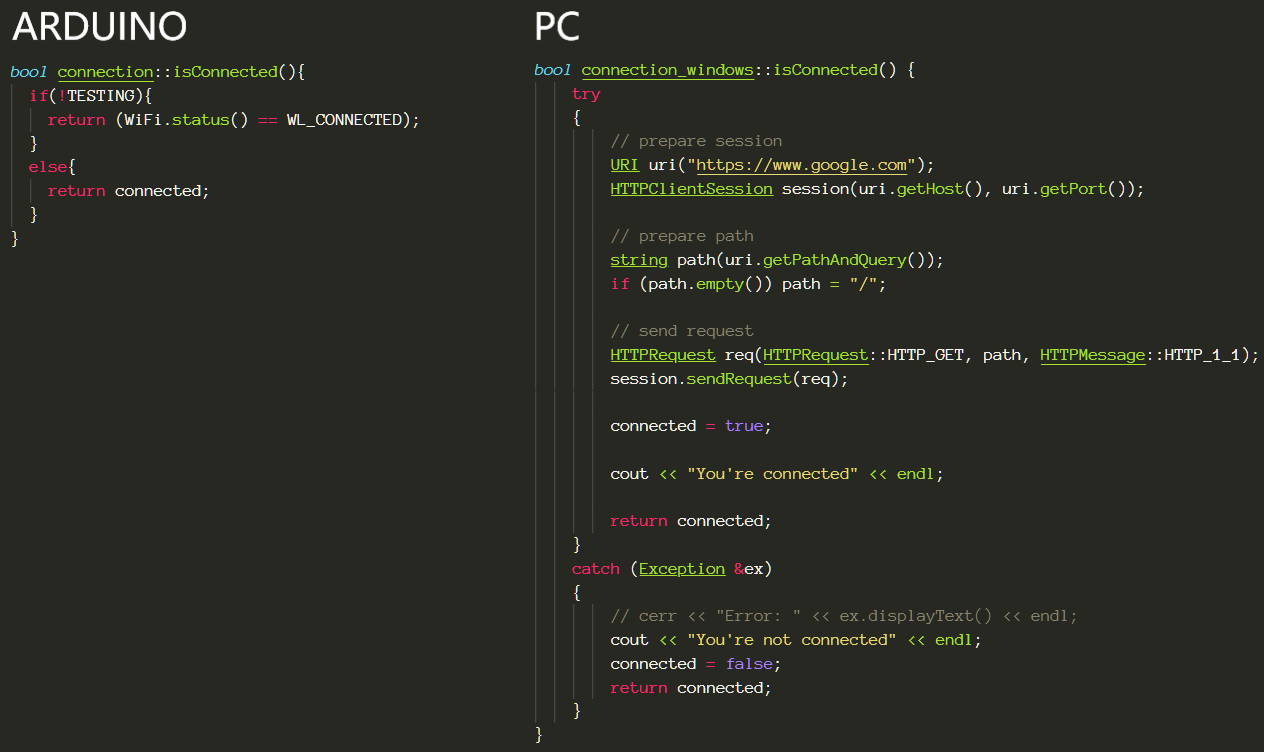
\includegraphics[width=\linewidth]{pics/connAW}
	\caption{Confronto tra le due implementazioni del metodo \textit{isConnected}}
	\label{connAW}
\end{figure}
\subsubsection{APIRest\_windows}

